We now switch our attention and ask: given two (symmetric) random matrices $A, B \ensuremath{\in} \ensuremath{\bbR}^{n \ensuremath{\times} n}$  and $B$, what are the distribution of the eigenvalues of $A+B$?  The rather remarkable fact is that, as $n \ensuremath{\rightarrow} \ensuremath{\infty}$,  if we know the global distribution of $A$ and $B$, in the form of knowing the moments $\ensuremath{\bm{\mathrm{E}}} A^k$ and $\ensuremath{\bm{\mathrm{E}}} B^k$, under very broad conditions we can deduce the global distribution of $A+B$, in the form of knowing the moments $\ensuremath{\bm{\mathrm{E}}} (A+B)^k$, where again we use
\[
\ensuremath{\bm{\mathrm{E}}} f(A) := \ensuremath{\bbE} \Tr f(A).
\]
The key observation is that $A$ and $B$, which do not in general commute ($AB \ensuremath{\neq} BA$), follow the rules of \emph{freely independent} non-commutative random variables. Thus the global statistics of $A+B$ can be thought of as a \emph{free convolution}, a non-commutative analogue of convolution. 

\section{Experimental observation of free convolutions}
We begin with an experimental observation of free convolution. Consider again a symmetric matrix $A_n \ensuremath{\in} \ensuremath{\bbR}^{n \ensuremath{\times} n}$  whose entries on and above the diagonal are iid random variables taking values $\ensuremath{\pm}1$ with equal probability. We saw in the previous chapter the global statistics are given by the semicircle. Now consider adding a diagonal matrix $D_n \ensuremath{\in} \ensuremath{\bbR}^{n \ensuremath{\times} n}$ with $\ensuremath{\pm}2$ on the diagonal with equal probability: what are the global statistics of $A_n + D_n$? We can explore this question numerically:


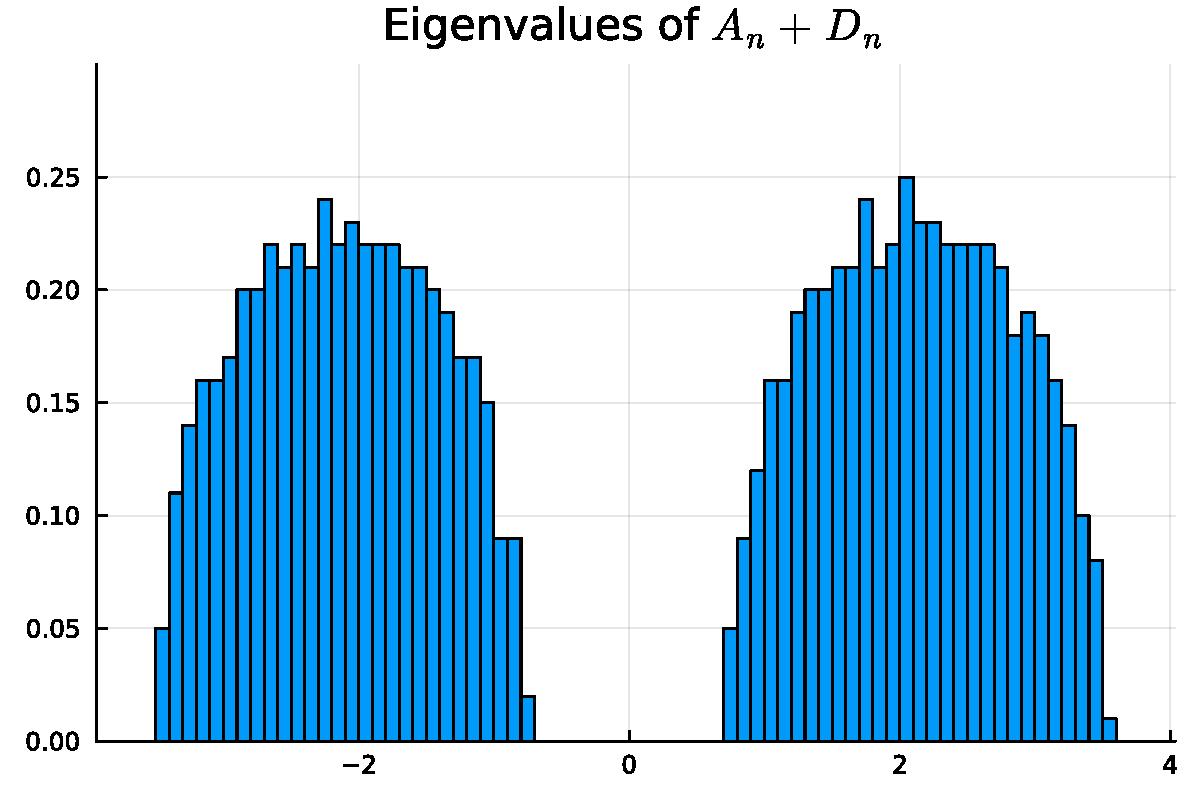
\includegraphics[width=0.6\linewidth,height=0.45\linewidth]{figures/II.FreeProbability_1_1.pdf}

We see that we get two semicircle-like distributions, surrounding \ensuremath{\pm}2. 

What's remarkable is this distribution only depends on the eigenvalues of $A_n$ and $D_n$. For example, consider the case where we same randomly $Q_n \ensuremath{\in} O(n)$, i.e., a random orthogonal matrix and define $B_n := Q_n D_n Q_n^\ensuremath{\top}$. This has exactly the same eigenvalues as $D_n$ itself. And when we add $A_n + B_n$ we get the exact same global statistics:


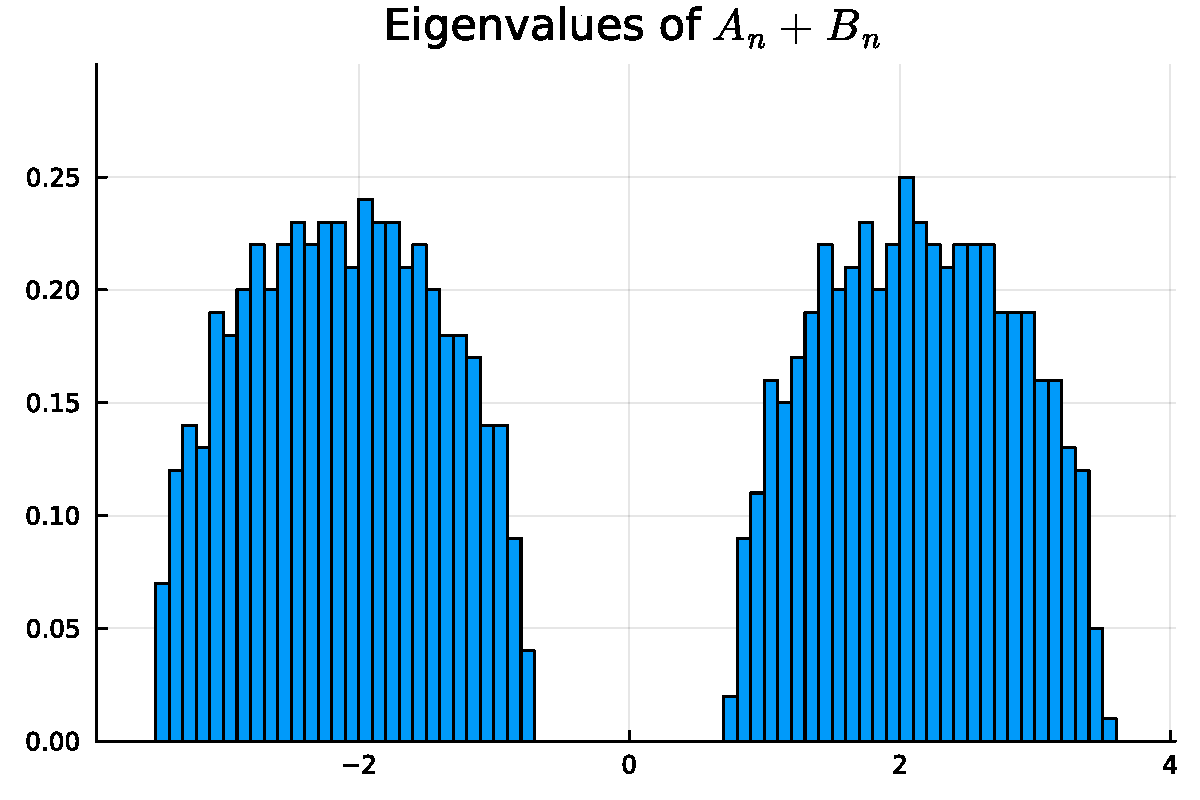
\includegraphics[width=0.6\linewidth,height=0.45\linewidth]{figures/II.FreeProbability_2_1.pdf}

This is a numerical demonstration of the fact that we can, under broad conditions, deduce the global eigenvalue statistics of $A_n + B_n$ from those of $A_n$ and $B_n$, and largely ignore the eigenvectors. To prove this we will again use the Method of Moments.

\section{Free random variables}
We put aside viewing $A$ and $B$ as random matrices and instead think of them more abstractly as \emph{free random variables}, which are non-commutative random variables which satisfy the following:

\begin{definition}[free random variables] $A$ and $B$ are \emph{free random variables} equipped with an expectation $\ensuremath{\bm{\mathrm{E}}}$ if for all polynomials $f_1,\ensuremath{\ldots},f_n$ and $g_1,\ensuremath{\ldots},g_n$ such that $\ensuremath{\bm{\mathrm{E}}} f_k(A) = \ensuremath{\bm{\mathrm{E}}} g_k(B) = 0$ we have
\[
\ensuremath{\bm{\mathrm{E}}} f_1(A) g_1(B) \ensuremath{\ldots} f_n(A) g_n(A) = 0,
\]
where the identity element satisfies $\ensuremath{\bm{\mathrm{E}}} I = 1$. \end{definition}

We claim (without proof) that as $n \ensuremath{\rightarrow} \ensuremath{\infty}$ that $\ensuremath{\bm{\mathrm{E}}} := \ensuremath{\bbE} \Tr$ behaves exactly like this for many families of random matrices. 

Note that we assume linearity: for constants $c,d$ we have
\[
\ensuremath{\bm{\mathrm{E}}} (c A + d B) = c \ensuremath{\bm{\mathrm{E}}}  A + d \ensuremath{\bm{\mathrm{E}}} B.
\]
It follows that (treating $\ensuremath{\bm{\mathrm{E}}}A^k$ as a constant)
\[
\ensuremath{\bm{\mathrm{E}}}(A^k - (\ensuremath{\bm{\mathrm{E}}}A^k) I ) =  \ensuremath{\bm{\mathrm{E}}} A^k - \ensuremath{\bm{\mathrm{E}}}A^k \ensuremath{\bm{\mathrm{E}}}I  = 0.
\]
This simple observation guarantees that if we know the moments $\ensuremath{\bm{\mathrm{E}}} A^k$ and $\ensuremath{\bm{\mathrm{E}}} B^k$ we can deduce the moments $\ensuremath{\bm{\mathrm{E}}} A^k B^j$. To see this, we first consider some of the low order cases. First, we note that by subtracting off the free expectation of moments of $A$ and $B$ and treating $\ensuremath{\bm{\mathrm{E}}}[A^k], \ensuremath{\bm{\mathrm{E}}}[B^j]$ as constants we deduce:
\meeq{
0 = \ensuremath{\bm{\mathrm{E}}}[(A^k-\ensuremath{\bm{\mathrm{E}}}[A^k] I) (B^j-\ensuremath{\bm{\mathrm{E}}}[B^j] I)] =\ensuremath{\bm{\mathrm{E}}}[A^k B^j] - \ensuremath{\bm{\mathrm{E}}}A^k \ensuremath{\bm{\mathrm{E}}}B^j \qquad \ensuremath{\Rightarrow} \ccr
\ensuremath{\bm{\mathrm{E}}}[A^k B^j] = \ensuremath{\bm{\mathrm{E}}}A^k \ensuremath{\bm{\mathrm{E}}}B^j
}
which is identical to classical random variables. This apparent consistency with classic random variables works for one mixed moment:
\meeq{
0 = \ensuremath{\bm{\mathrm{E}}}[(A-\ensuremath{\bm{\mathrm{E}}}[A] I) (B-\ensuremath{\bm{\mathrm{E}}}[B] I)(A-\ensuremath{\bm{\mathrm{E}}}[A] I)] \ccr
= 
\ensuremath{\bm{\mathrm{E}}}[ABA] - \ensuremath{\bm{\mathrm{E}}}[A] \ensuremath{\bm{\mathrm{E}}}[AB] - \ensuremath{\bm{\mathrm{E}}}[B]\ensuremath{\bm{\mathrm{E}}}[A^2] -\ensuremath{\bm{\mathrm{E}}}[A] \ensuremath{\bm{\mathrm{E}}}[BA]+2\ensuremath{\bm{\mathrm{E}}}[A]^2 \ensuremath{\bm{\mathrm{E}}}[B] \ccr
=
\ensuremath{\bm{\mathrm{E}}}[ABA] - \ensuremath{\bm{\mathrm{E}}}[B]\ensuremath{\bm{\mathrm{E}}}[A^2]\qquad \Rightarrow \ccr
\ensuremath{\bm{\mathrm{E}}}[ABA] = \ensuremath{\bm{\mathrm{E}}}[A^2]\ensuremath{\bm{\mathrm{E}}}[B]
}
where we use $\ensuremath{\bm{\mathrm{E}}}[AB] = \ensuremath{\bm{\mathrm{E}}}[A] \ensuremath{\bm{\mathrm{E}}}[B]$.  But that's where the equivalence ends. In particular, consider:
\meeq{
0 = \ensuremath{\bm{\mathrm{E}}}[(A-\ensuremath{\bm{\mathrm{E}}}[A] I) (B-\ensuremath{\bm{\mathrm{E}}}[B] I)(A-\ensuremath{\bm{\mathrm{E}}}[A] I) (B-\ensuremath{\bm{\mathrm{E}}}[B] I) ]\ccr
 = 
\ensuremath{\bm{\mathrm{E}}}[ABAB] - \underbrace{\ensuremath{\bm{\mathrm{E}}}[ABA]}_{=\ensuremath{\bm{\mathrm{E}}}[A^2]\ensuremath{\bm{\mathrm{E}}}[B]}  \ensuremath{\bm{\mathrm{E}}}[B] -\ensuremath{\bm{\mathrm{E}}}[A] \underbrace{\ensuremath{\bm{\mathrm{E}}}[A B^2]}_{=\ensuremath{\bm{\mathrm{E}}}[A] \ensuremath{\bm{\mathrm{E}}}[B^2]}  + \underbrace{\ensuremath{\bm{\mathrm{E}}}[AB]}_{=\ensuremath{\bm{\mathrm{E}}}[A]\ensuremath{\bm{\mathrm{E}}}[B]} \ensuremath{\bm{\mathrm{E}}}[A] \ensuremath{\bm{\mathrm{E}}}[B]\\
&\qquad - \underbrace{\ensuremath{\bm{\mathrm{E}}}[A^2B]}_{=\ensuremath{\bm{\mathrm{E}}}[A^2]\ensuremath{\bm{\mathrm{E}}}[B]} \ensuremath{\bm{\mathrm{E}}}[B] + \ensuremath{\bm{\mathrm{E}}}[A^2] \ensuremath{\bm{\mathrm{E}}}[B]^2 + \underbrace{\ensuremath{\bm{\mathrm{E}}}[A B]}_{=\ensuremath{\bm{\mathrm{E}}}[A]\ensuremath{\bm{\mathrm{E}}}[B]} \ensuremath{\bm{\mathrm{E}}}[A] \ensuremath{\bm{\mathrm{E}}}[B] - \ensuremath{\bm{\mathrm{E}}}[A]^2 \ensuremath{\bm{\mathrm{E}}}[B]^2\\
&\qquad - \ensuremath{\bm{\mathrm{E}}}[A] \underbrace{\ensuremath{\bm{\mathrm{E}}}[BA B]}_{=\ensuremath{\bm{\mathrm{E}}}[A] \ensuremath{\bm{\mathrm{E}}}[B^2]} + \ensuremath{\bm{\mathrm{E}}}[A] \ensuremath{\bm{\mathrm{E}}}[B]\underbrace{\ensuremath{\bm{\mathrm{E}}}[BA]}_{=\ensuremath{\bm{\mathrm{E}}}[A]\ensuremath{\bm{\mathrm{E}}}[B]}  + \ensuremath{\bm{\mathrm{E}}}[A]^2 \ensuremath{\bm{\mathrm{E}}}[B^2] - \ensuremath{\bm{\mathrm{E}}}[A]^2 \ensuremath{\bm{\mathrm{E}}}[B]^2\\
&\qquad + \ensuremath{\bm{\mathrm{E}}}[A] \ensuremath{\bm{\mathrm{E}}}[B]\underbrace{\ensuremath{\bm{\mathrm{E}}}[AB]}_{=\ensuremath{\bm{\mathrm{E}}}[A]\ensuremath{\bm{\mathrm{E}}}[B]} - \ensuremath{\bm{\mathrm{E}}}[A]^2 \ensuremath{\bm{\mathrm{E}}}[B]^2  - \ensuremath{\bm{\mathrm{E}}}[A]^2 \ensuremath{\bm{\mathrm{E}}}[B]^2 +  \ensuremath{\bm{\mathrm{E}}}[A]^2 \ensuremath{\bm{\mathrm{E}}}[B]^2 \ccr
= \ensuremath{\bm{\mathrm{E}}}[ABAB] - \ensuremath{\bm{\mathrm{E}}}[A^2] \ensuremath{\bm{\mathrm{E}}}[B]^2 - \ensuremath{\bm{\mathrm{E}}}[A]^2 \ensuremath{\bm{\mathrm{E}}}[B^2] + \ensuremath{\bm{\mathrm{E}}}[A]^2 \ensuremath{\bm{\mathrm{E}}}[B]^2 \qquad \Rightarrow \ccr
\ensuremath{\bm{\mathrm{E}}}[ABAB] = \ensuremath{\bm{\mathrm{E}}}[A^2] \ensuremath{\bm{\mathrm{E}}}[B]^2 + \ensuremath{\bm{\mathrm{E}}}[A]^2 \ensuremath{\bm{\mathrm{E}}}[B^2] - \ensuremath{\bm{\mathrm{E}}}[A]^2 \ensuremath{\bm{\mathrm{E}}}[B]^2
}
which differs from the classical (commutative) case  where $\ensuremath{\bm{\mathrm{E}}}[ABAB] = \ensuremath{\bm{\mathrm{E}}}[A^2] \ensuremath{\bm{\mathrm{E}}}[B^2]$. Nevertheless, we can see the central theme emerging: $\ensuremath{\bm{\mathrm{E}}}[ABAB]$ is still given in terms of a function of the input moments $\ensuremath{\bm{\mathrm{E}}}[A^k]$ and $\ensuremath{\bm{\mathrm{E}}}[B^j]$.

\section{Free convolution}
\section{Poster projects}

